\section{Método da Pesquisa}
%\use o comando "\columnbreak", para quebrar o final da 1º coluna, caso necessite
%Digite a baixo o seu referencial teórico
As atividades do projeto de pesquisa iniciaram-se no mês de maio de 2019 nas dependências da sede provisória do IFPB – Campus Santa Luzia. Dentre as etapas estabelecidas no cronograma proposto no projeto a primeira ação foi a realização de uma apresentação do projeto para os participantes, com a finalidade de esclarecer os seus reais objetivos e metas almejadas pelo projeto.\par
No que se refere ao cumprimento das demandas listadas no cronograma, inicialmente foi realizada a oficina de eletricidade e eletrônica básica, a qual teve como objetivo expor e apresentar aos alunos conceito referentes a grandezas, medidas elétricas e dispositivos eletrônicos através de aulas teóricas e práticas.

\subsection{Capacitação: eletricidade e eletrônica}
As oficinas de eletricidade e eletrônica buscaram preparar os alunos para o manuseio de dispositivos elétricos, tornando-os capazes de montar circuitos elétricos simples; realizar medidas elétrica; interpretar esquemas elétricos; associar componentes elétricos de forma correta. Uma vez que para manusear a plataforma Arduino os alunos necessitam do referido conhecimento prévio.
\textbf{INCLUIR REFERÊNCIAL TEÓRICO}

\begin{figure}[H] % !htbh esolhe a melhor posição para inserir a figura
    \centering %figura centralizada
    \caption{Caption}
    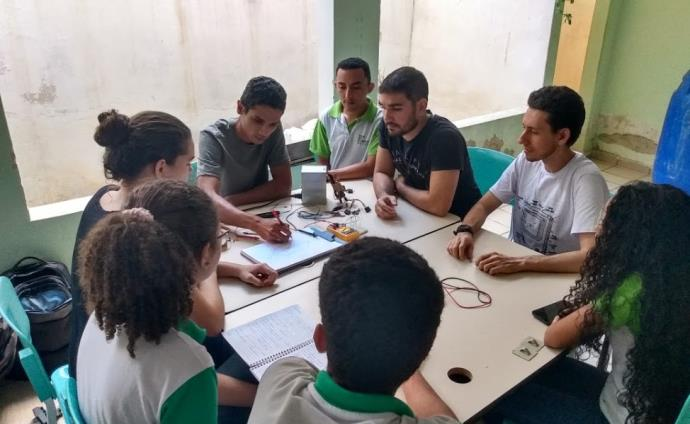
\includegraphics[scale=0.3]{lib/figuras/aula1_eletrica_eletronica.png}
    \\
    {\footnotesize Fonte: Autor próprio.}
    \label{fig:aula01_eletrica}
\end{figure}

\subsection{}